\documentclass{IEEEcsmag}

\usepackage[colorlinks,urlcolor=blue,linkcolor=blue,citecolor=blue]{hyperref}
\expandafter\def\expandafter\UrlBreaks\expandafter{\UrlBreaks\do\/\do\*\do\-\do\~\do\'\do\"\do\-}
\usepackage{upmath,color}
\usepackage{multirow}
\usepackage[table,xcdraw]{xcolor}


\jvol{00}
\jnum{00}
\paper{8}
\jmonth{May}
\jname{}
\jtitle{}
\pubyear{2023}

\newtheorem{theorem}{Theorem}
\newtheorem{lemma}{Lemma}


\setcounter{secnumdepth}{0}

\begin{document}

\sptitle{Empirical Study}

\title{On the maintenability of ECS and Object-Oriented programming in video games, an empirical study}

\author{Billy Bouchard}
\affil{Polytechnique Montréal, Montréal, QC, Canada}

\markboth{THEME/FEATURE/DEPARTMENT}{THEME/FEATURE/DEPARTMENT}

%\begin{abstract}\looseness-1

%end{abstract}

\maketitle


\chapteri{}

\section{Introduction}

Video game development has always been a world where performance dictates the bests.
Since the creation of DOOM up to the newest Assasins Creed, we try to squash every bit of performance from both the CPU and GPU to obtain the best graphics, realistic AIs, accurate physics and a fluid experience for the player. to achieve this effect, so many different architectures have been implemented and tested. For example, Doom used a model-based approach, Unreal engine uses a superclass architecture and Unity uses a component base architecture. However, all of these have been developed with performance as the core concern. All of these use Object Oriented Programming as the way to go to develop the games.

However, recently, data-oriented programming, more specifically ECS or Entity-Component-System, has surfaced as the newest and most performant architecture one can use to develop video games. A couple of solutions have come out most notable of which being the DOTS framework offered by Unity which just recently launch the 1.0 version. Some notorious game that used such engine includes Overwatch, Fortnite, Hearthstone and Star Citizen. As more and more actors in the industry start to use it, it becomes important to better understand this framework to make better use of it.

It is important to note, that while ECS is considered a great programming framework, most of the games that use it do not exclusively use it. Consequently, object oriented-programming might still be used in a lot of those projects.

Software engineering has developed a great number of methods in object-oriented programing to make programs more maintainable. From video game-specific architecture to video game-specific design patterns. However, not as much work and research has been put into the different facets of ECS and how it truly compares to the industry-approved 

in this work, I shall focus on the maintainability of video games project focusing on ECS. As to understand how maintainability specifically affects ECS, I had to find a way to know. With the overwhelming amount of video game projects that are there, it became possible that simply comparing ECS projects with other types of video game projects would let me know how they compare. This study is intended as an initiation to see if the average ECS project is more maintainable than  other video game architecture.

\section{Related Work}


\section{Methodology}


This paper tries to better understand ECS projects and the maintainability of such programs. To attain this effect,  I will use object-oriented programing (OOP) as the baseline from which the ECS framework shall be compared. Since the industry has used OOP a lot, it will be easier to see what place ECS takes, and how it performs. my first research question is: 
\begin{quote}
    RQ0. ECS architecture does not work with common video games architectures
\end{quote}

To answer this question, I had to find a couple of repositories that used mostly or completely the ECS framework. To find the repositories, I searched open-source projects on GitHub with the keyword "Entity ", "Component" and "System". All projects that did not have at least 100 commits were discarded as they were not mature enough to be considered. Some  ECS projects could have a portion of the code written using another architecture. Therefore, to be considered, I manually check the project and made sure they were ECS-centric (meaning at least half of the files were used to create components or systems or to manage those. Therefore, this part was subjective. I decided that plugin repositories would be considered as long as their architecture respected ECS with the same rules that any video game repositories were following (more than 100 commits). Since a manual verification was needed, only the 5 most forkable projects would be kept for comparison.

Then for further comprehension, a control group was needed. This control group needed to not use ECS and be a well-known engine in the video game world. I simply used the "video game" keyword for my search through GitHub and then selected the top forked game engine and all the open-source game engines I found an ECS plugin for. I applied the same rules to find interesting repositories: they had to have at least 100 commits to be considered and I only kept the ones with the most forks. 

Once repository selection was completed, I looked into two different metrics. The first one will be the change-proness defined as the frequency of a file to be changed. The conclusion we are trying to observe led to RQ1. 

\begin{quote}
    RQ1. The average change-proness does not change in ECS projects from the average video game project.
\end{quote}

To calculate this metric, we will look at the average amount of change in a commit from any project from its creation to its last version. Since longer projects will tend to have more changes but also more commit, this shall represent fairly the change-proness.
equation : 

\begin{equation}
    changeproness = \frac{TotalFileChanges}{nbCommits} 
\end{equation}

To get this information, I will use an automated approach that will count the number of changes in each commit of the projects. A file being present in a commit means it has been either created, modified (Changed) or destroyed. A simple ratio will tell me how much changes by file, and then, an average shall tell me the change-proness of the whole project. We then will be able to find if the ratio of changes is higher or lower in ECS base projects. 

the second section will look at the faultproness of files. this meant RQ2.

\begin{quote}
    RQ2. The average faultproness does not change in ECS projects from the average video game project.
\end{quote}

To make it simple, faultproness is the number of bugs created in a program. However, since a lot of bugs are not known, I needed to find a way to count most of the bugs or at least the important ones. I search for the commits that fixed bugs (the ones with the keywords "bug" or "fix" in it) to get a fair estimate of the number of bugs in the lifecycle of the program. Finding the ratio of change intended to correct bugs over every commit will give us a quick overview of how much effort was put into bug fixing over feature addition or modification. The smaller the ratio the less bugfix is needed per feature.

\begin{equation}
    faultproness = \frac{TotalBugFixFilesChanges}{TotalFileChanges}
\end{equation}


%\begin{figure}
%\centerline{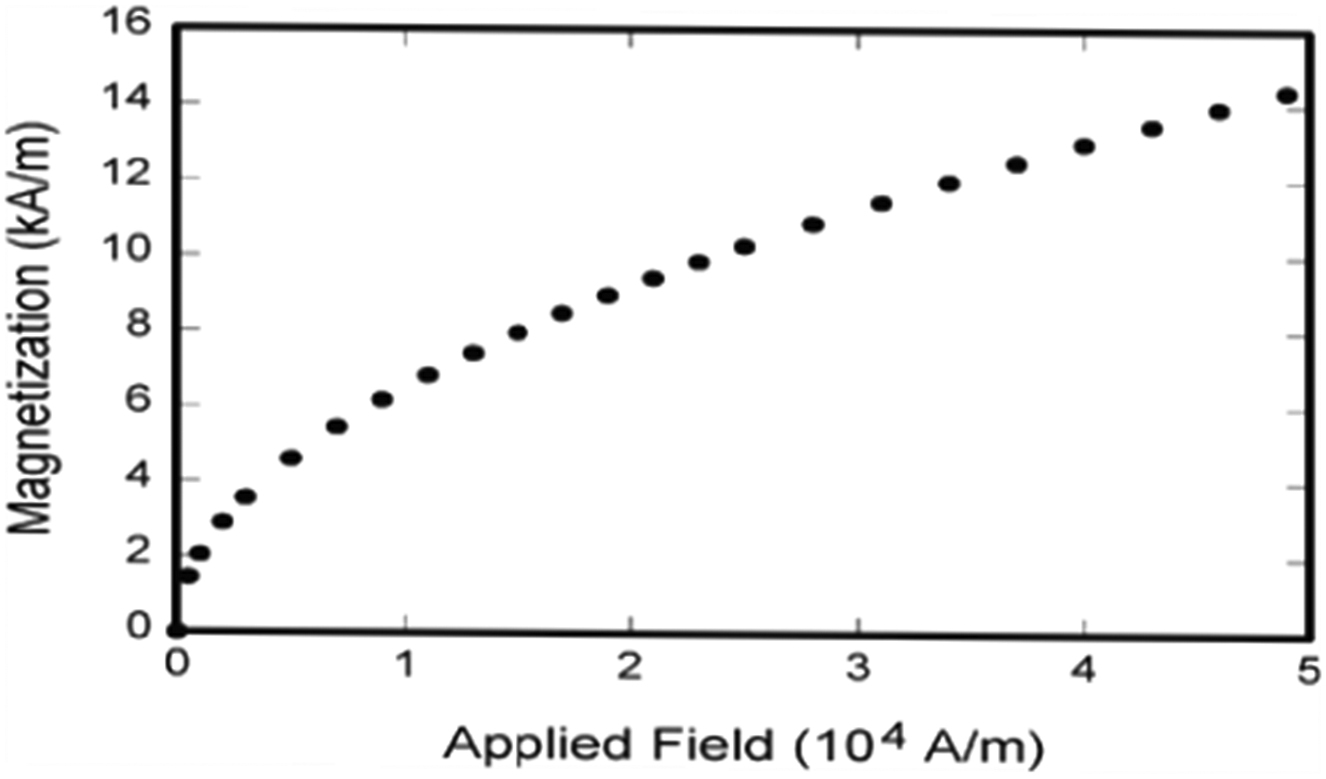
\includegraphics[width=18.5pc]{fig1.jpg}}
%\caption{Note that ``Figure'' is spelled out. There is a period after the figure number, followed by one space. It is good practice to briefly explain the significance of the figure in the caption. (From [``Title''],$^1$ used with permission.)}\vspace*{-5pt}
%\end{figure}


\section{Results}
\begin{table}[]
    \begin{tabular}{|l|l|l|}
        \hline
        \cellcolor[HTML]{000000} & Engine      & Link                                       \\ \hline
                                 & Godex       & https://github.com/GodotECS/godex          \\ \cline{2-3} 
                                 & Entt        & https://github.com/skypjack/entt           \\ \cline{2-3} 
                                 & flecs       & https://github.com/SanderMertens/flecs     \\ \cline{2-3} 
                                 & Entitas     & https://github.com/JuDelCo/Entitas-Cpp     \\ \cline{2-3} 
        \multirow{-5}{*}{ECS}    & Uecs        & https://github.com/Ubpa/UECS               \\ \hline
                                 & Godot       & https://github.com/godotengine/godot       \\ \cline{2-3} 
                                 & Pixijs      & https://github.com/pixijs/pixijs           \\ \cline{2-3} 
                                 & Babylon     & https://github.com/BabylonJS/Babylon.js    \\ \cline{2-3} 
                                 & OpenDiablo2 & https://github.com/OpenDiablo2/OpenDiablo2 \\ \cline{2-3} 
        \multirow{-5}{*}{Others} & Minetest    & https://github.com/minetest/minetest       \\ \hline
    \end{tabular}
    \caption{Chosen repositories and links}
\end{table}

Finding the repositories was easier than anticipated since I had experience with a lot of different video game engines and knew quite my share about ECS-based engines. Therefore, however subjective my analysis was, I was able to decern the true marking of an ECS engine from the top research prospect. I was mostly looking at an architecture that encouraged the usage of Components and Systems. That led me to 5 well-known plugins that anyone who dwelled a bit into video game ECS development would know and that are presented in Table 1. From those plugins, I directly went and found the open-source game engine linked to them. this led me to find the GODOT engine. All the other game engines found were well-known. Using the fork amount made a lot of sense in the context of video game engines since the more forks there were, the more projects using the engine there are. This enables us to refute the null hypothesis RQ0. A lot of ECS engine does use a basic Object Oriented framework to work. The best example of which being the Godot ECS plugin Godex. 

% Please add the following required packages to your document preamble:
% \usepackage{multirow}
% \usepackage[table,xcdraw]{xcolor}
% If you use beamer only pass "xcolor=table" option, i.e. \documentclass[xcolor=table]{beamer}
% Please add the following required packages to your document preamble:
% \usepackage{multirow}
% \usepackage[table,xcdraw]{xcolor}
% If you use beamer only pass "xcolor=table" option, i.e. \documentclass[xcolor=table]{beamer}
\begin{table}[]
    \begin{tabular}{|
    >{\columncolor[HTML]{FFFFFF}}l |
    >{\columncolor[HTML]{FFFFFF}}l |
    >{\columncolor[HTML]{FFFFFF}}l |
    >{\columncolor[HTML]{FFFFFF}}l |
    >{\columncolor[HTML]{FFFFFF}}l |}
    \hline
    \cellcolor[HTML]{000000} &
      \cellcolor[HTML]{000000}{\color[HTML]{000000} } &
      {\color[HTML]{000000} commits} &
      {\color[HTML]{000000} \begin{tabular}[c]{@{}l@{}}file \\ changes\end{tabular}} &
      \begin{tabular}[c]{@{}l@{}}Change-\\ pronness\end{tabular} \\ \hline
    \cellcolor[HTML]{FFFFFF}                         & {\color[HTML]{000000} Godex}       & {\color[HTML]{000000} 490} & {\color[HTML]{000000} 358086}  & 730.79  \\ \cline{2-5} 
    \cellcolor[HTML]{FFFFFF}                         & {\color[HTML]{000000} Entt}        & {\color[HTML]{000000} 490} & {\color[HTML]{000000} 71324}   & 145.56  \\ \cline{2-5} 
    \cellcolor[HTML]{FFFFFF}                         & {\color[HTML]{000000} flecs}       & {\color[HTML]{000000} 490} & {\color[HTML]{000000} 1554265} & 3171.97 \\ \cline{2-5} 
    \cellcolor[HTML]{FFFFFF}                         & {\color[HTML]{000000} Entitas}     & {\color[HTML]{000000} 490} & {\color[HTML]{000000} 157360}  & 321.14  \\ \cline{2-5} 
    \cellcolor[HTML]{FFFFFF}                         & {\color[HTML]{000000} UECS}        & {\color[HTML]{000000} 253} & {\color[HTML]{000000} 48129}   & 190.23  \\ \cline{2-5} 
    \multirow{-6}{*}{\cellcolor[HTML]{FFFFFF}ECS}    & {\color[HTML]{000000} Average}     & {\color[HTML]{000000} 443} & {\color[HTML]{000000} 437833}  & 911.94  \\ \hline
    \cellcolor[HTML]{FFFFFF}                         & {\color[HTML]{000000} Godot}       & {\color[HTML]{000000} 490} & {\color[HTML]{000000} 233644}  & 476.82  \\ \cline{2-5} 
    \cellcolor[HTML]{FFFFFF}                         & {\color[HTML]{000000} Pixijs}      & {\color[HTML]{000000} 490} & {\color[HTML]{000000} 374859}  & 765.02  \\ \cline{2-5} 
    \cellcolor[HTML]{FFFFFF}                         & {\color[HTML]{000000} Babylon}     & {\color[HTML]{000000} 490} & {\color[HTML]{000000} 47650}   & 97.24   \\ \cline{2-5} 
    \cellcolor[HTML]{FFFFFF}                         & {\color[HTML]{000000} OpenDiablo2} & {\color[HTML]{000000} 490} & {\color[HTML]{000000} 51565}   & 105.23  \\ \cline{2-5} 
    \cellcolor[HTML]{FFFFFF}                         & {\color[HTML]{000000} minetest}    & {\color[HTML]{000000} 490} & {\color[HTML]{000000} 251732}  & 513.74  \\ \cline{2-5} 
    \multirow{-6}{*}{\cellcolor[HTML]{FFFFFF}Others} & {\color[HTML]{000000} Average}     & {\color[HTML]{000000} 490} & {\color[HTML]{000000} 191890}  & 391.61  \\ \hline
    \end{tabular}
    \caption{Change-pronness of the different repositories}
\end{table}

The sheer amount of commits every repository had made it so that an upper limit had to be drawn to enable me to finally get some results. For example, the principal Godot repositories had over 53k commits. With the simple GitHub API token given to me, I was only able to process 5k commits per hour. This would have resulted in over a day to get all the results from all the repositories. Since I did not have the time to do all that and that a simple poorly done code line could have brought me back to square 0,  I decided to subsample. Instead, I focus on the most recent 500 commits of each repo. I was then able to find the change-proness of each repository with the simple formula given at the start. Results are shown in Table 2. Flecs seems to be out of place with more than a million changes. All the other repositories however seemed to share the average range of changes by commit. All of that stopped us from refuting our null hypothesis RQ1.

% Please add the following required packages to your document preamble:
% \usepackage{multirow}
% \usepackage[table,xcdraw]{xcolor}
% If you use beamer only pass "xcolor=table" option, i.e. \documentclass[xcolor=table]{beamer}
\begin{table}[]
    \begin{tabular}{|
    >{\columncolor[HTML]{FFFFFF}}l |
    >{\columncolor[HTML]{FFFFFF}}l |
    >{\columncolor[HTML]{FFFFFF}}l |
    >{\columncolor[HTML]{FFFFFF}}l |
    >{\columncolor[HTML]{FFFFFF}}l |}
    \hline
    \cellcolor[HTML]{000000}{\color[HTML]{000000} } &
      \cellcolor[HTML]{000000}{\color[HTML]{000000} } &
      {\color[HTML]{000000} \begin{tabular}[c]{@{}l@{}}file \\ changes\end{tabular}} &
      {\color[HTML]{000000} \begin{tabular}[c]{@{}l@{}}file \\ changes \\ in fix \\ commits\end{tabular}} &
      {\color[HTML]{000000} Faultproness} \\ \hline
    \cellcolor[HTML]{FFFFFF}{\color[HTML]{000000} } &
      {\color[HTML]{000000} Godex} &
      {\color[HTML]{000000} 358086} &
      {\color[HTML]{000000} 10073} &
      {\color[HTML]{000000} 2.81\%} \\ \cline{2-5} 
    \cellcolor[HTML]{FFFFFF}{\color[HTML]{000000} } &
      {\color[HTML]{000000} Entt} &
      {\color[HTML]{000000} 71324} &
      {\color[HTML]{000000} 46} &
      {\color[HTML]{000000} 0.06\%} \\ \cline{2-5} 
    \cellcolor[HTML]{FFFFFF}{\color[HTML]{000000} } &
      {\color[HTML]{000000} flecs} &
      {\color[HTML]{000000} 1554265} &
      {\color[HTML]{000000} 720756} &
      {\color[HTML]{000000} 46.37\%} \\ \cline{2-5} 
    \cellcolor[HTML]{FFFFFF}{\color[HTML]{000000} } &
      {\color[HTML]{000000} Entitas} &
      {\color[HTML]{000000} 157360} &
      {\color[HTML]{000000} 13662} &
      {\color[HTML]{000000} 8.68\%} \\ \cline{2-5} 
    \cellcolor[HTML]{FFFFFF}{\color[HTML]{000000} } &
      {\color[HTML]{000000} UECS} &
      {\color[HTML]{000000} 48129} &
      {\color[HTML]{000000} 2535} &
      {\color[HTML]{000000} 5.27\%} \\ \cline{2-5} 
    \multirow{-6}{*}{\cellcolor[HTML]{FFFFFF}{\color[HTML]{000000} ECS}} &
      {\color[HTML]{000000} Average} &
      {\color[HTML]{000000} 437833} &
      {\color[HTML]{000000} 149414} &
      {\color[HTML]{000000} 12.64\%} \\ \hline
    \cellcolor[HTML]{FFFFFF}{\color[HTML]{000000} } &
      {\color[HTML]{000000} Godot} &
      {\color[HTML]{000000} 233644} &
      {\color[HTML]{000000} 9378} &
      {\color[HTML]{000000} 4.01\%} \\ \cline{2-5} 
    \cellcolor[HTML]{FFFFFF}{\color[HTML]{000000} } &
      {\color[HTML]{000000} Pixijs} &
      {\color[HTML]{000000} 374859} &
      {\color[HTML]{000000} 11072} &
      {\color[HTML]{000000} 2.95\%} \\ \cline{2-5} 
    \cellcolor[HTML]{FFFFFF}{\color[HTML]{000000} } &
      {\color[HTML]{000000} Babylon} &
      {\color[HTML]{000000} 47650} &
      {\color[HTML]{000000} 7511} &
      {\color[HTML]{000000} 15.76\%} \\ \cline{2-5} 
    \cellcolor[HTML]{FFFFFF}{\color[HTML]{000000} } &
      {\color[HTML]{000000} OpenDiablo2} &
      {\color[HTML]{000000} 51565} &
      {\color[HTML]{000000} 12058} &
      {\color[HTML]{000000} 23.38\%} \\ \cline{2-5} 
    \cellcolor[HTML]{FFFFFF}{\color[HTML]{000000} } &
      {\color[HTML]{000000} minetest} &
      {\color[HTML]{000000} 251732} &
      {\color[HTML]{000000} 4205} &
      {\color[HTML]{000000} 1.67\%} \\ \cline{2-5} 
    \multirow{-6}{*}{\cellcolor[HTML]{FFFFFF}{\color[HTML]{000000} Others}} &
      {\color[HTML]{000000} Average} &
      {\color[HTML]{000000} 191890} &
      {\color[HTML]{000000} 8845} &
      {\color[HTML]{000000} 9.56\%} \\ \hline
    \end{tabular}
    \caption{Fault pronness of the different repositories}
\end{table}

The last statistic that we wanted to see was faultproness. I used a naive approach that let me simply get the percentage of commits that focus on bug fixes out of the total amount of changes. This led to the percentage shown in Table 3. Same as for table 2, Flecs seems to be anomalous data that does not bring clear information to the table. It has about 10 times more changes than the average repo, thus giving us a bad representation of the ECS base code. Because of this, it is not possible to refute hypothesis RQ2.

\section{Discussion}

As sad as it was to find strongly anomalous data, it is still possible to find something out of the remainder data. Consequently, we examine both Godot repository and its ECS plugin Godex. both had over 500 commits and can therefore be fairly well compared. Godex being newer and having fewer commits, it made sense for it to have the most changes by commit. around 1.7 times more changes. However, when looking at the most recent commits, and therefore at the ones who should try to tackle the most bug, we discover that fault seems to appear 1% less in Godex, the ECS plugin. However, in itself, it is not enough to conclude. Entt is another great case study as it probably is the most known ECS engine on the open-source market, rivalled only by Unity DOTS technology, which is proprietary software and therefore can't be analysed in this study. Seeing that over the 500 commits, there were almost no bugs and only feature addition or removal let us think that ECS might be more maintainable. However, all these statistics seem to lack just a bit to prove that ECS is also a more maintainable architecture than the other architecture used in video games. From my perspective, it seems like change-proness (or at least my way of calculating it) does not seem to be affected by the architecture. However, although impossible to achieve a clear conclusion, data does point toward fault-proness being a little bit smaller in ECS base architecture. The thing that blocks us from that conclusion is Flecs' results, which gave us a whopping 50% fault ratio. 

This study needed to manually find the repositories that would be studied since there are no tools that I know of which let one knows if a repository is really of ECS architecture. Therefore, it limited my ability to find more data. We were able to prove that almost all ECS project does begin in some way, not as direct data-oriented programming, but in part as object-oriented programming. It makes sense too, as a lot of ECS engines/plugins are made to work on well-known video game architecture like Unity or Unreal Engine. 

\section{Validity}

This research had validity issues that I tried to mitigate. The first one is the fact that I was alone in my search. However easier it might get, since I don't have to argue with anyone over what I deem most important, it can also lead me to have focused on the wrong part.  It could also lead me to not have considered every important aspect of the problem. It also led me to have a subjective view that could not be challenged by colleagues. To mitigate this, I tried to automate a lot of my techniques and diminish to a minimum the amount of subjective part of the study. I focus on formulas that could give me the info I needed. When subjectivity was indeed needed, I used GitHub algorithm to present me with the best possible solution and went from top to bottom.    

Construct validity, it regards the tools used for this study. My main tool was GitHub and its API. Since GitHub is the biggest tool to manage and find open-source repositories, it made sense to use it instead of any other. Due to time constraints as well as resources constraint, I had to find the website that would give me the most information. I also used a Python script to collect information from GitHub. This script is accessible in the replication package provided one enters its own GitHub API token. To generate the script I used a base script generated by chat GPT which I modified to suit my needs.

External validity regards how generalizable this study can be. With the way information was grabbed,  this study is highly reproducible. This can be redone simply using the scripts given as part of the replication package. If one wanted to find other repositories, the method with which the repositories were fetched is well explained in the methodology section. A lot of the programs used had way over 500 commits. The whole study took place on a total of 5k commits which should be enough to see tendencies. Moreover, all plugins and video game engines were considered without regard to the language but only based on the quality of their repository.

\section{Conclusion}

This study aimed at demonstrating that maintaining ECS architecture was at worst as easy as maintaining any other video game program. We first demonstrated that ECS was usually part of a bigger architecture and rarely by itself. This was through a simple search that demonstrated that repositories like Godex depended on other engines to work (GODOT in this case). Then we tried to search for a link between change-proneness and ECS. This was really without any conclusion as all the repositories both from ECS and the control group had a, what seemed random, amount of changes by commit.  Following this, we tried to prove that fault-proneness appears less often in ECS base programs. However, Flecs, which seemed to be anomalous data, falsify any conclusion we could make. Further investigation, however, could prove a tendency for ECS to be less fault-prone.

Of course, the subject of video game development does need a lot more presence. ECS is the up-and-coming architecture and will take an increasing place in the video game development world. Studies need to find what can make their development harder. This will help teams better plan their usage of ECS.

\def\refname{REFERENCES}

\begin{thebibliography}{1}

\bibitem{AA1}
Gamma, E., Helm, R., Johnson, R.,, Vlissides, J. M. (1994). Design Patterns: Elements of Reusable Object-Oriented Software. Addison-Wesley Professional. ISBN: 0201633612

\bibitem{BB1}
Ceruzzi, P. E. (2003). A history of modern computing. MIT press.

\bibitem{CC1}
Wexelblat, R. L. (Ed.). (2014). History of programming languages. Academic Press.

\bibitem{DD1}
Hansen, H., \& Öhrström, O. (2020). Benchmarking and Analysis of Entity Referencing Within Open-Source Entity Component Systems.

\bibitem{EE1}
Kafaji, K. (2018, March 29). Entity Component System in Unity: An Introduction. Ray Wenderlich. https://www.raywenderlich.com/847-entity-component-system-in-unity-an-introduction

\bibitem{FF1}
Nystrom, R. (2014). Game Programming Patterns. Chapter 12: Entity Component System. Genever Benning. https://gameprogrammingpatterns.com/component.html

\bibitem{HH1}
ECSTY. (n.d.). Retrieved May 3, 2023, from https://ecsy.io/

\bibitem{II1}
Vittoria Nardone, Biruk Asmare Muse, Mouna Abidi, Foutse Khomh, and Massimiliano Di Penta. 2022. Video Game Bad Smells: What they are and how Developers Perceive Them. ACM Trans. Softw. Eng. Methodol. Just Accepted (September 2022). https://doi.org/10.1145/3563214

\end{thebibliography}
\end{document}

